% !TeX root = document.tex
% !TeX encoding = UTF-8 Unicode

\section{Results}%
\label{sec:results}

\subsection{Level System}%
\label{subsec:level-system}

\begin{slide}{System Description}
  \vspace*{\fill}
  \begin{figure}[ht!]
    \centering
    \captionsetup{justification=centering}
    \tikzset{every picture/.style={line width=0.75pt}}
    \resizebox{!}{0.75\textheight}{%
        \tikzset{every picture/.style={line width=0.75pt}} %set default line width to 0.75pt        
    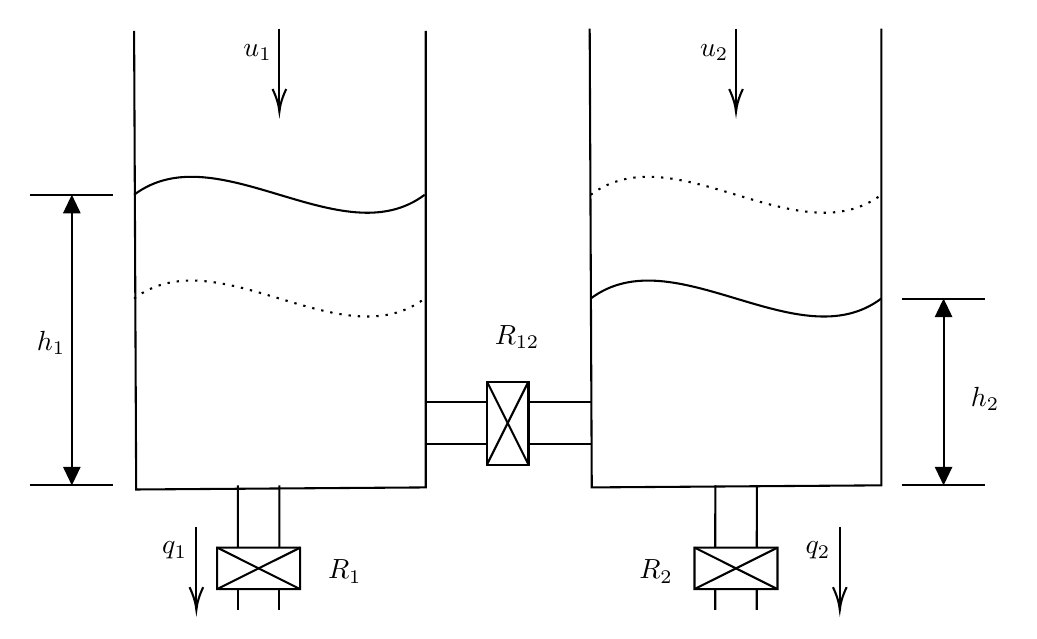
\begin{tikzpicture}[x=0.75pt,y=0.75pt,yscale=-1,xscale=1]
        %uncomment if require: \path (0,459); %set diagram left start at 0, and has height of 459
        %Straight Lines [id:da5688929335924803] 
        \draw    (310.5,121) -- (310.5,341) -- (171,342) -- (170,121) ;
        %Straight Lines [id:da5444294116492245] 
        \draw    (530,120) -- (530,340) -- (390.5,341) -- (389.5,120) ;
        %Straight Lines [id:da5805131124126722] 
        \draw    (200,360) -- (200,398) ;
        \draw [shift={(200,400)}, rotate = 270] [color={rgb, 255:red, 0; green, 0; blue, 0 }  ][line width=0.75]    (10.93,-3.29) .. controls (6.95,-1.4) and (3.31,-0.3) .. (0,0) .. controls (3.31,0.3) and (6.95,1.4) .. (10.93,3.29)   ;
        %Straight Lines [id:da36945578968673487] 
        \draw    (510,360) -- (510,398) ;
        \draw [shift={(510,400)}, rotate = 270] [color={rgb, 255:red, 0; green, 0; blue, 0 }  ][line width=0.75]    (10.93,-3.29) .. controls (6.95,-1.4) and (3.31,-0.3) .. (0,0) .. controls (3.31,0.3) and (6.95,1.4) .. (10.93,3.29)   ;
        %Straight Lines [id:da3077937138084411] 
        \draw    (310,300) -- (340,300) ;
        %Straight Lines [id:da6773172185122848] 
        \draw    (310,320) -- (340,320) ;
        %Shape: Rectangle [id:dp35476624369345366] 
        \draw   (340,290) -- (360,290) -- (360,330) -- (340,330) -- cycle ;
        %Straight Lines [id:da9030142425581202] 
        \draw    (360,300) -- (390,300) ;
        %Straight Lines [id:da9329287059080266] 
        \draw    (360,320) -- (390,320) ;
        %Straight Lines [id:da7833363422326105] 
        \draw    (340,290) -- (360,330) ;
        %Straight Lines [id:da26540765973372593] 
        \draw    (360,290) -- (340,330) ;
        %Straight Lines [id:da7238601427391023] 
        \draw    (470.02,340) -- (470,370) ;
        %Straight Lines [id:da21192498383993508] 
        \draw    (450.02,339.99) -- (450,369.99) ;
        %Shape: Rectangle [id:dp4746471043409347] 
        \draw   (480,370.01) -- (479.99,390.01) -- (439.99,389.98) -- (440,369.98) -- cycle ;
        %Straight Lines [id:da6336671048955647] 
        \draw    (470,389.99) -- (469.98,400) ;
        %Straight Lines [id:da6700066277567417] 
        \draw    (450,389.99) -- (449.98,400) ;
        %Straight Lines [id:da928718960478936] 
        \draw    (480,370.01) -- (439.99,389.98) ;
        %Straight Lines [id:da1540497075962557] 
        \draw    (479.99,390.01) -- (440,369.98) ;
        %Straight Lines [id:da7575667165517417] 
        \draw    (240.03,340.01) -- (240.01,370.01) ;
        %Straight Lines [id:da24987185404211631] 
        \draw    (220.03,340) -- (220.01,370) ;
        %Shape: Rectangle [id:dp2771887371908066] 
        \draw   (250.01,370.02) -- (250,390.02) -- (210,389.99) -- (210.01,369.99) -- cycle ;
        %Straight Lines [id:da9912034440398235] 
        \draw    (240,390) -- (240,400) ;
        %Straight Lines [id:da11904000202181764] 
        \draw    (220,390) -- (220,400) ;
        %Straight Lines [id:da7480508238760858] 
        \draw    (250.01,370.02) -- (210,389.99) ;
        %Straight Lines [id:da7049908339863217] 
        \draw    (250,390.02) -- (210.01,369.99) ;
        %Straight Lines [id:da9101133488343268] 
        \draw    (240,120) -- (240,158) ;
        \draw [shift={(240,160)}, rotate = 270] [color={rgb, 255:red, 0; green, 0; blue, 0 }  ][line width=0.75]    (10.93,-3.29) .. controls (6.95,-1.4) and (3.31,-0.3) .. (0,0) .. controls (3.31,0.3) and (6.95,1.4) .. (10.93,3.29)   ;
        %Straight Lines [id:da11474588029910615] 
        \draw    (460,120) -- (460,158) ;
        \draw [shift={(460,160)}, rotate = 270] [color={rgb, 255:red, 0; green, 0; blue, 0 }  ][line width=0.75]    (10.93,-3.29) .. controls (6.95,-1.4) and (3.31,-0.3) .. (0,0) .. controls (3.31,0.3) and (6.95,1.4) .. (10.93,3.29)   ;
        %Curve Lines [id:da10596831311641142] 
        \draw    (170,200) .. controls (210,170) and (270,230) .. (310,200) ;
        %Curve Lines [id:da32042097611565956] 
        \draw    (390,250) .. controls (430,220) and (490,280) .. (530,250) ;
        %Curve Lines [id:da9628648357071894] 
        \draw  [dash pattern={on 0.84pt off 2.51pt}]  (170,250) .. controls (210,220) and (270,280) .. (310,250) ;
        %Curve Lines [id:da13605436176729158] 
        \draw  [dash pattern={on 0.84pt off 2.51pt}]  (390,200) .. controls (430,170) and (490,230) .. (530,200) ;
        %Straight Lines [id:da6375240487876032] 
        \draw    (140,202) -- (140,338) ;
        \draw [shift={(140,340)}, rotate = 270] [fill={rgb, 255:red, 0; green, 0; blue, 0 }  ][line width=0.75]  [draw opacity=0] (8.93,-4.29) -- (0,0) -- (8.93,4.29) -- cycle    ;
        \draw [shift={(140,200)}, rotate = 90] [fill={rgb, 255:red, 0; green, 0; blue, 0 }  ][line width=0.75]  [draw opacity=0] (8.93,-4.29) -- (0,0) -- (8.93,4.29) -- cycle    ;
        %Straight Lines [id:da08454244898673535] 
        \draw    (120,200) -- (160,200) ;
        %Straight Lines [id:da6622529040678575] 
        \draw    (120,340) -- (160,340) ;
        %Straight Lines [id:da8094387172838741] 
        \draw    (560,252) -- (560,338) ;
        \draw [shift={(560,340)}, rotate = 270] [fill={rgb, 255:red, 0; green, 0; blue, 0 }  ][line width=0.75]  [draw opacity=0] (8.93,-4.29) -- (0,0) -- (8.93,4.29) -- cycle    ;
        \draw [shift={(560,250)}, rotate = 90] [fill={rgb, 255:red, 0; green, 0; blue, 0 }  ][line width=0.75]  [draw opacity=0] (8.93,-4.29) -- (0,0) -- (8.93,4.29) -- cycle    ;
        %Straight Lines [id:da5524739963534533] 
        \draw    (540,250) -- (580,250) ;
        %Straight Lines [id:da7800336719151444] 
        \draw    (540,340) -- (580,340) ;
        % Text Node
        \draw (189.5,371.5) node  [align=left] {$\displaystyle q_{1}$};
        % Text Node
        \draw (499.5,371.5) node  [align=left] {$\displaystyle q_{2}$};
        % Text Node
        \draw (354.5,268.5) node  [align=left] {$\displaystyle R_{12}$};
        % Text Node
        \draw (229.5,131.5) node  [align=left] {$\displaystyle u_{1}$};
        % Text Node
        \draw (449.5,131.5) node  [align=left] {$\displaystyle u_{2}$};
        % Text Node
        \draw (130,271.5) node  [align=left] {$\displaystyle h_{1}$};
        % Text Node
        \draw (580,298.5) node  [align=left] {$\displaystyle h_{2}$};
        % Text Node
        \draw (271.5,381.5) node  [align=left] {$\displaystyle R_{1}$};
        % Text Node
        \draw (421.5,381.5) node  [align=left] {$\displaystyle R_{2}$};
    \end{tikzpicture}%
    }
    \caption{System of Coupled Tanks}%
    \label{fig:tanks-sim}
\end{figure}

  \vspace*{\fill}
\end{slide}

\begin{slide}{System Description}
  \vspace*{\fill}
  \begin{columns}[T]
    \begin{column}{0.48\textwidth}
      \begin{equation}
        \label{eq:formula-height-variation-lin}
        \begin{aligned}
          \dot{h}_1(t) & = \frac{u_1(t)-q_1(t)\pm{}q_{12}}{A},   \\
          \dot{h}_2(t) & = \frac{u_2(t)-q_2(t)\mp{}q_{12}}{A},   \\
          q_1(t)       & = a\sqrt{2gh_1(t)},                     \\
          q_2(t)       & = a\sqrt{2gh_2(t)},                     \\
          q_{12}(t)    & = a\sqrt{2g\left|h_2(t)-h_1(t)\right|}.
        \end{aligned}
      \end{equation}
    \end{column}%
    \hfill%
    \begin{column}{0.48\textwidth}
      \begin{equation}
        \begin{aligned}
          x_{eq}^1 & = \begin{bmatrix}
            57.5 \\ 43.61
          \end{bmatrix} \\
          u_{eq}^1 & = \begin{bmatrix}
            744 \\ 2960
          \end{bmatrix} \\
          x_{eq}^2 & = \begin{bmatrix}
            43.61 \\ 57.5
          \end{bmatrix} \\
          u_{eq}^2 & = \begin{bmatrix}
            2960 \\ 744
          \end{bmatrix}
        \end{aligned}
      \end{equation}
    \end{column}%
  \end{columns}
  \vspace*{\fill}
\end{slide}

\begin{slide}{System Description}
  \vspace*{\fill}
  \begin{columns}[T]
    \begin{column}{0.38\textwidth}
      \begin{equation}
        \begin{aligned}
          A_1 & =
          \begin{bmatrix}
            0.92  & 0.053 \\
            0.053 & 0.91
          \end{bmatrix},          \\
          A_2 & = \begin{bmatrix}
            0.91  & 0.053 \\
            0.053 & 0.92
          \end{bmatrix}   \\
          B_1 & =
          \begin{bmatrix}
            0.0016           & 4.5\times10^{-5} \\
            4.5\times10^{-5} & 0.0016
          \end{bmatrix},          \\
          B_2 & = \begin{bmatrix}
            0.0016           & 4.5\times10^{-5} \\
            4.5\times10^{-5} & 0.0016
          \end{bmatrix}, \\
          C_1 & = C_2 =
          \begin{bmatrix}
            1 & 0 \\
            0 & 1
          \end{bmatrix}.
        \end{aligned}
      \end{equation}
    \end{column}
    \hfill%
    \begin{column}{0.58\textwidth}
      \begin{equation}
        \begin{aligned}
          K_1 & = \begin{bmatrix}
            -875.384 & -9.217   & -297.447 & 7.982    \\
            -8.505   & -849.853 & 8.514    & -279.434
          \end{bmatrix}, \\
          K_2 & = \begin{bmatrix}
            -849.853 & -8.505   & -279.434 & 8.514    \\
            -9.217   & -875.384 & 7.982    & -297.447
          \end{bmatrix}.
        \end{aligned}
      \end{equation}
    \end{column}%
    %
  \end{columns}
  \vspace*{\fill}
\end{slide}

\begin{slide}{System Description}
  \vspace*{\fill}
  \begin{figure}[ht!]
    \centering
    \captionsetup{justification=centering}
    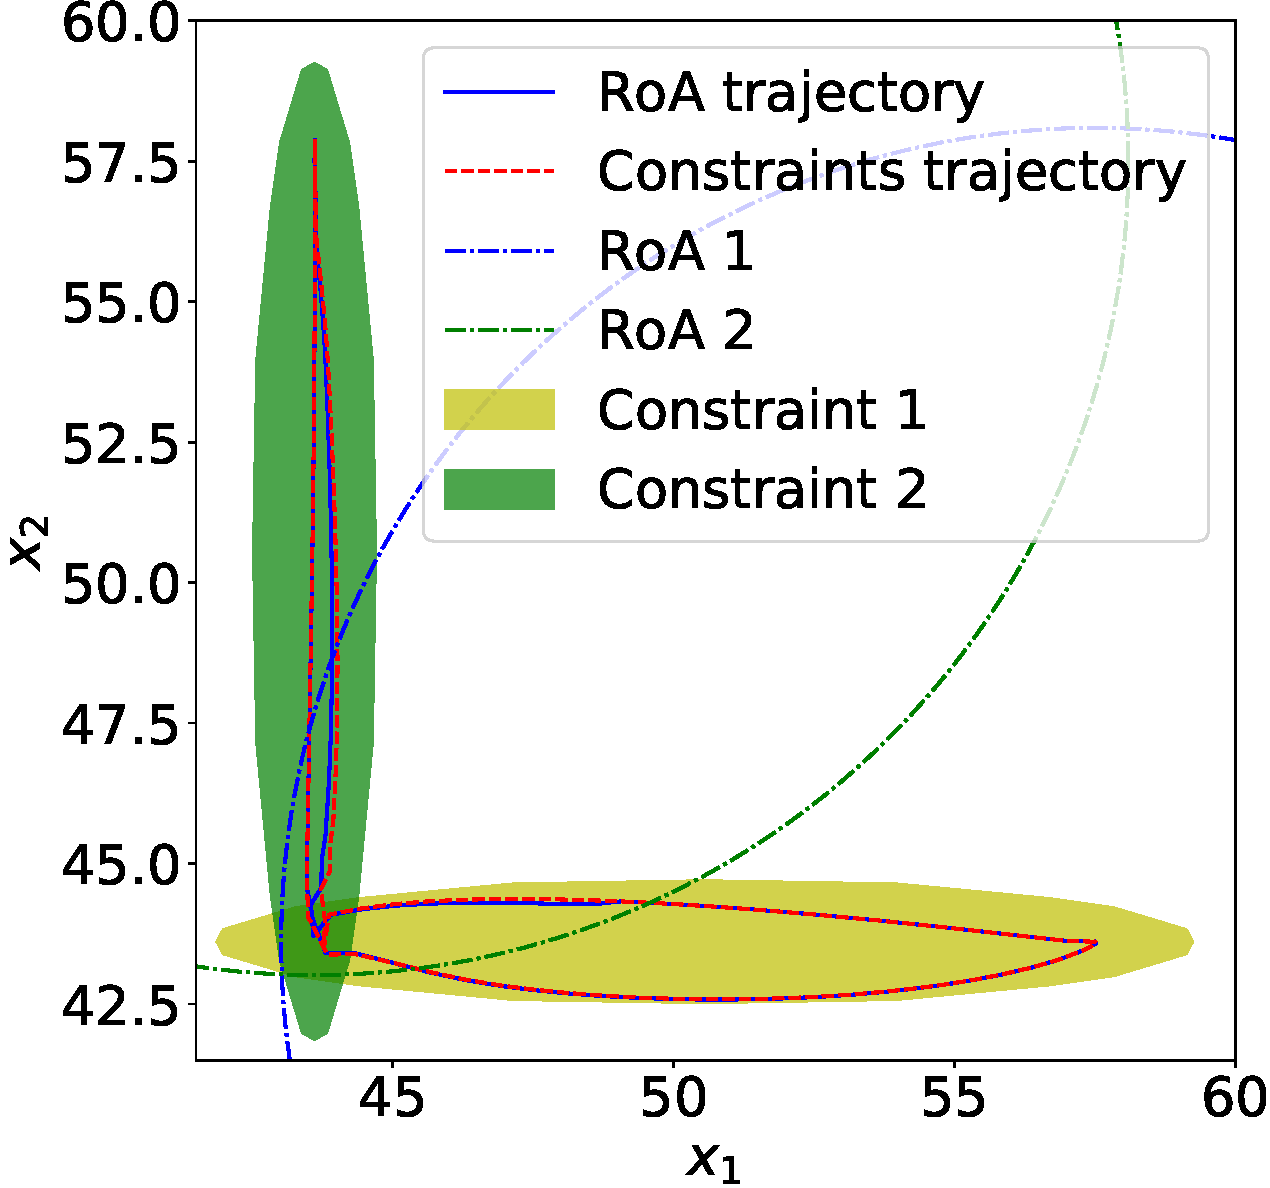
\includegraphics[height=0.75\textheight]{tanks-states}
    \caption{States trajectory for Example 1.}%
    \label{fig:level-system-control-states}
  \end{figure}
  \vspace*{\fill}
\end{slide}

\begin{slide}{System Description}
  \vspace*{\fill}
  \begin{figure}[ht!]
    \centering
    \captionsetup{justification=centering}
    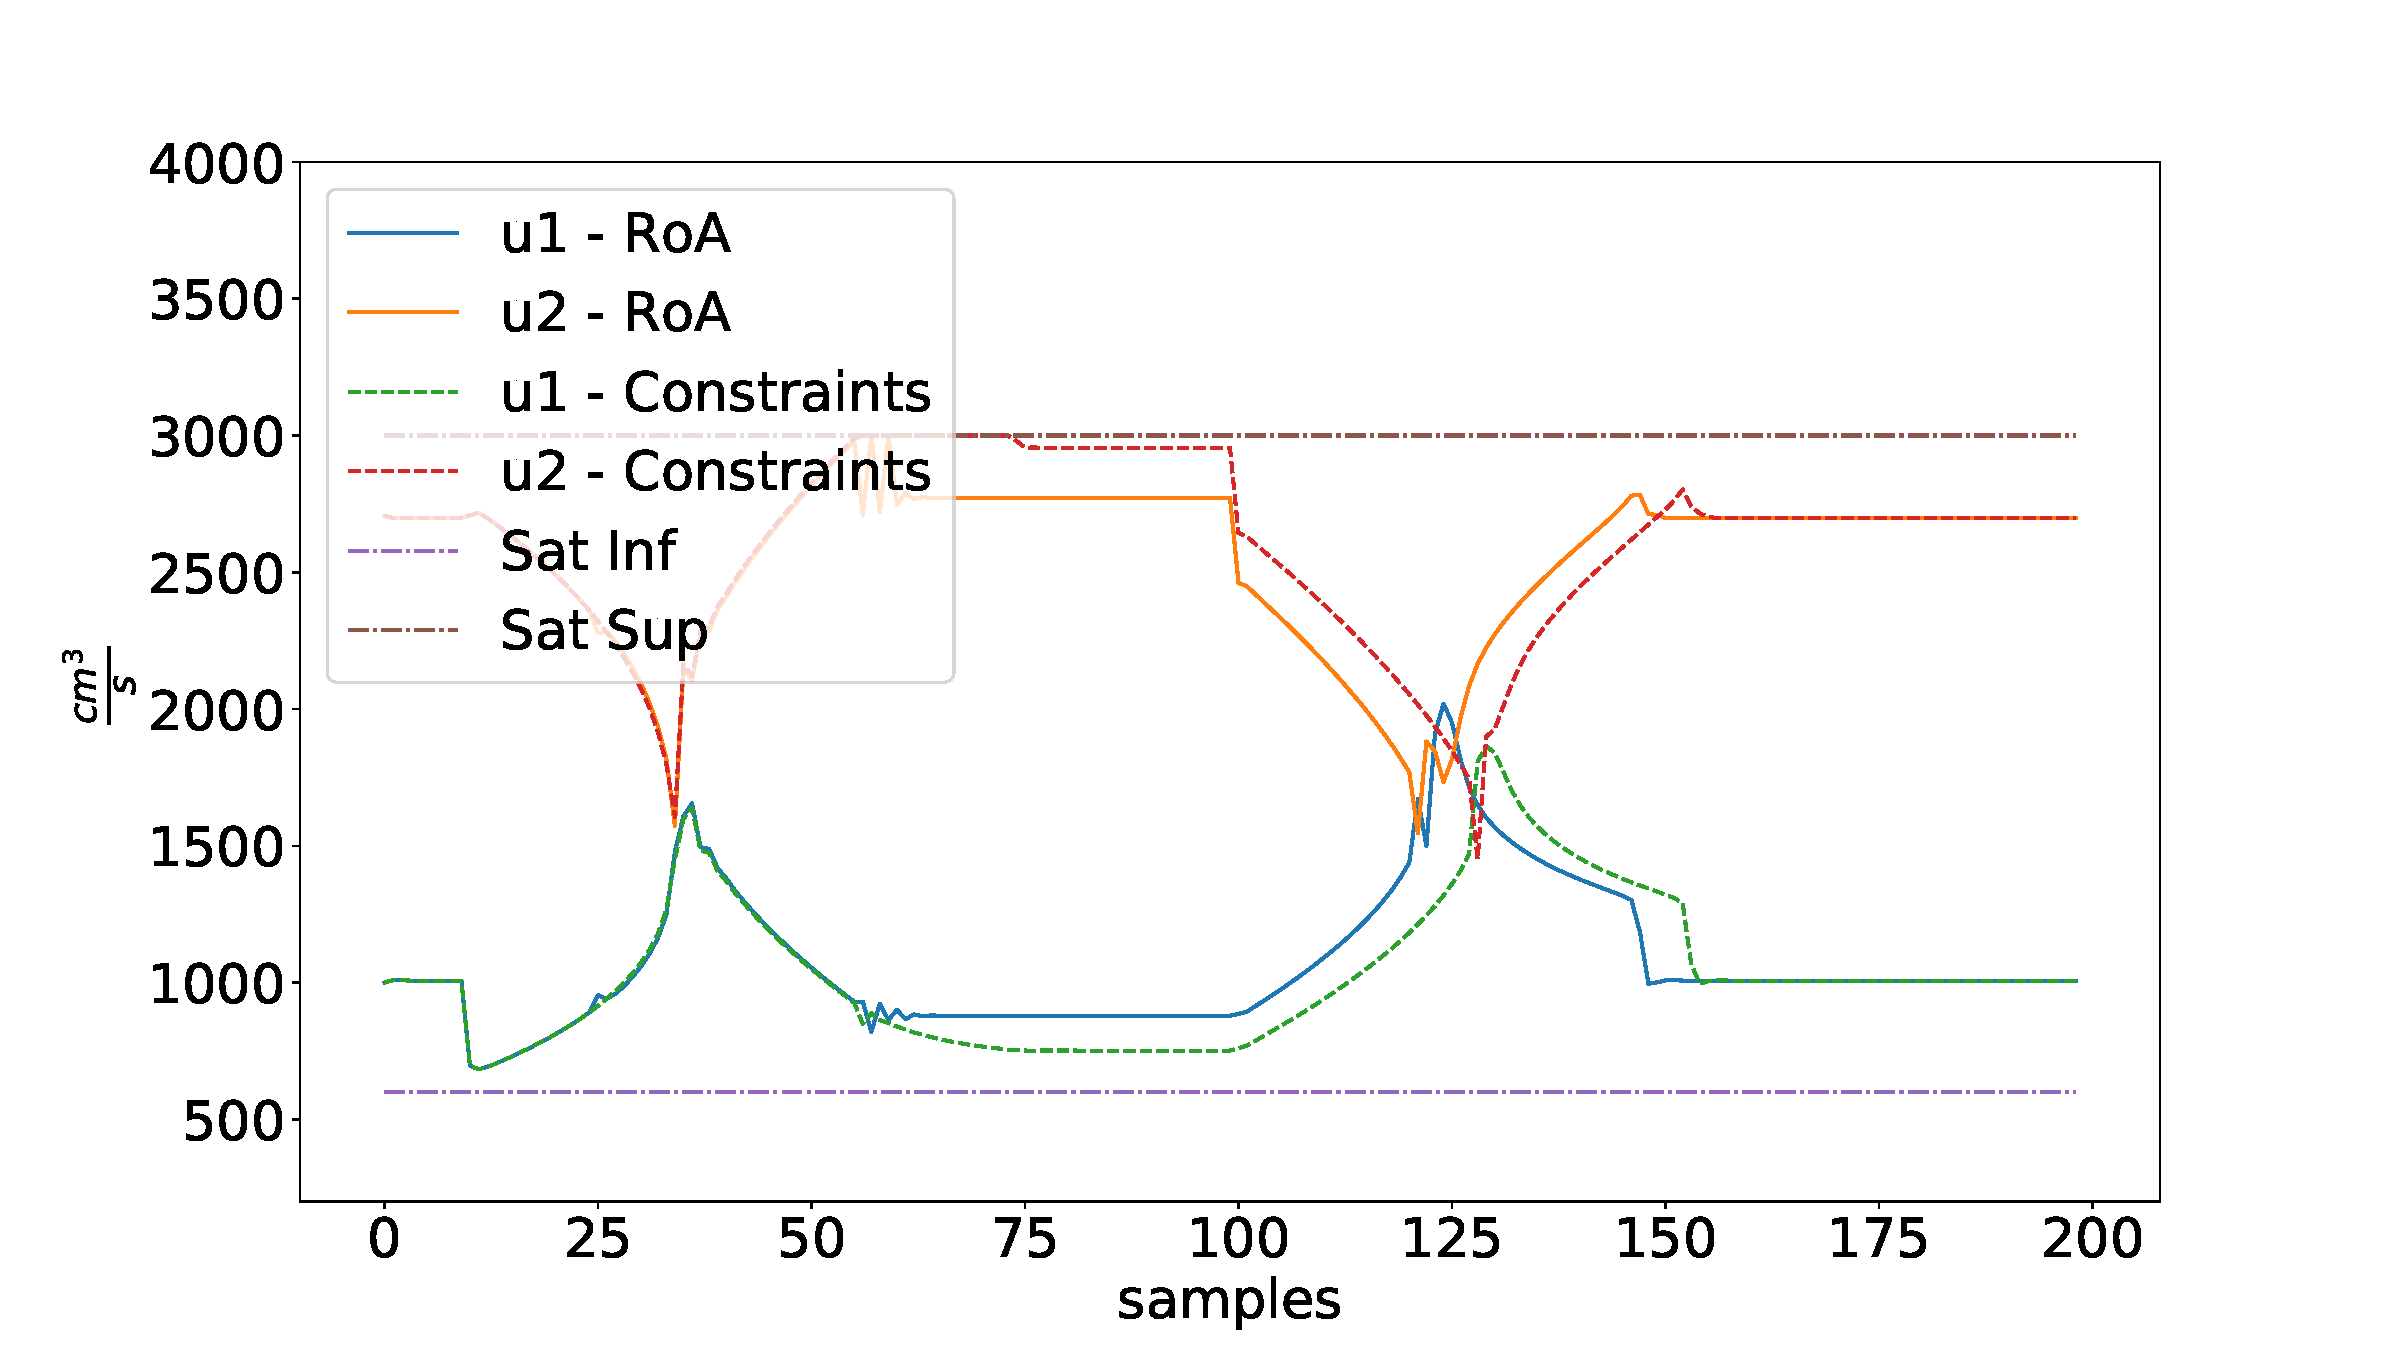
\includegraphics[height=0.75\textheight]{tanks-control-signal}
    \caption{Control signals for Example 1.}%
    \label{fig:level-system-control-signals}
  \end{figure}
  \vspace*{\fill}
\end{slide}

\subsection{Unstable System}%
\label{subsec:unstable-system}

\begin{slide}{Goal of Command Governor}
  \vspace*{\fill}
  \begin{columns}[T]
    \begin{column}{0.38\textwidth}
      \begin{equation}
        \begin{aligned}
          A_1 & =
          \begin{bmatrix}
            1 & 0.003 \\
            0 & 1
          \end{bmatrix}          \\
          A_2 & = \begin{bmatrix}
            1 & 0.0074 \\
            0 & 1.1
          \end{bmatrix}, \\
          B_1 & =
          \begin{bmatrix}
            0.0005 & 1.2\times{}10^{-6} \\
            0      & 0.0008
          \end{bmatrix},         \\
          B_2 & = \begin{bmatrix}
            0.0019 & 3.6\times{}10^{-5} \\
            0      & 0.011
          \end{bmatrix}, \\
          %
          C_1 & = C_2 =
          \begin{bmatrix}
            1 & 0 \\
            0 & 1
          \end{bmatrix}.         \\
        \end{aligned}
      \end{equation}
    \end{column}%
    \hfill%
    \begin{column}{0.58\textwidth}
      \begin{equation}
        \begin{aligned}
          x_{eq}^1 = \begin{bmatrix}
            1 \\ 1
          \end{bmatrix},
          u_{eq}^1 = \begin{bmatrix}
            -2 \\ \frac{-5}{4}
          \end{bmatrix},
          x_{eq}^2 = \begin{bmatrix}
            -1 \\ 1
          \end{bmatrix},
          u_{eq}^2 = \begin{bmatrix}
            \frac{-30}{19} \\ -10
          \end{bmatrix}.
        \end{aligned}
      \end{equation}
      \begin{equation}
        \resizebox{0.8\linewidth}{!}{%
          \(\begin{aligned}
            K_1 & = \begin{bmatrix}
              -2.669\times{}10^3   & -1.993             & -6.741\times{}10^2    & 1.010              \\
              3.582\times{}10^{-4} & -1.669\times{}10^3 & -3.103\times{}10^{-4} & -4.210\times{}10^2
            \end{bmatrix}, \\
            K_2 & = \begin{bmatrix}
              -7.034\times{}10^2    & -1.268             & -1.769\times{}10^2    & 6.097\times{}10^{-1} \\
              -3.903\times{}10^{-6} & -1.370\times{}10^2 & -1.292\times{}10^{-5} & -3.202\times{}10^1
            \end{bmatrix}.
          \end{aligned}\)
        }
      \end{equation}
    \end{column}%
  \end{columns}
  \vspace*{\fill}
\end{slide}

\begin{slide}{Goal of Command Governor}
  \vspace*{\fill}
  \begin{figure}[ht!]
    \centering
    \captionsetup{justification=centering}
    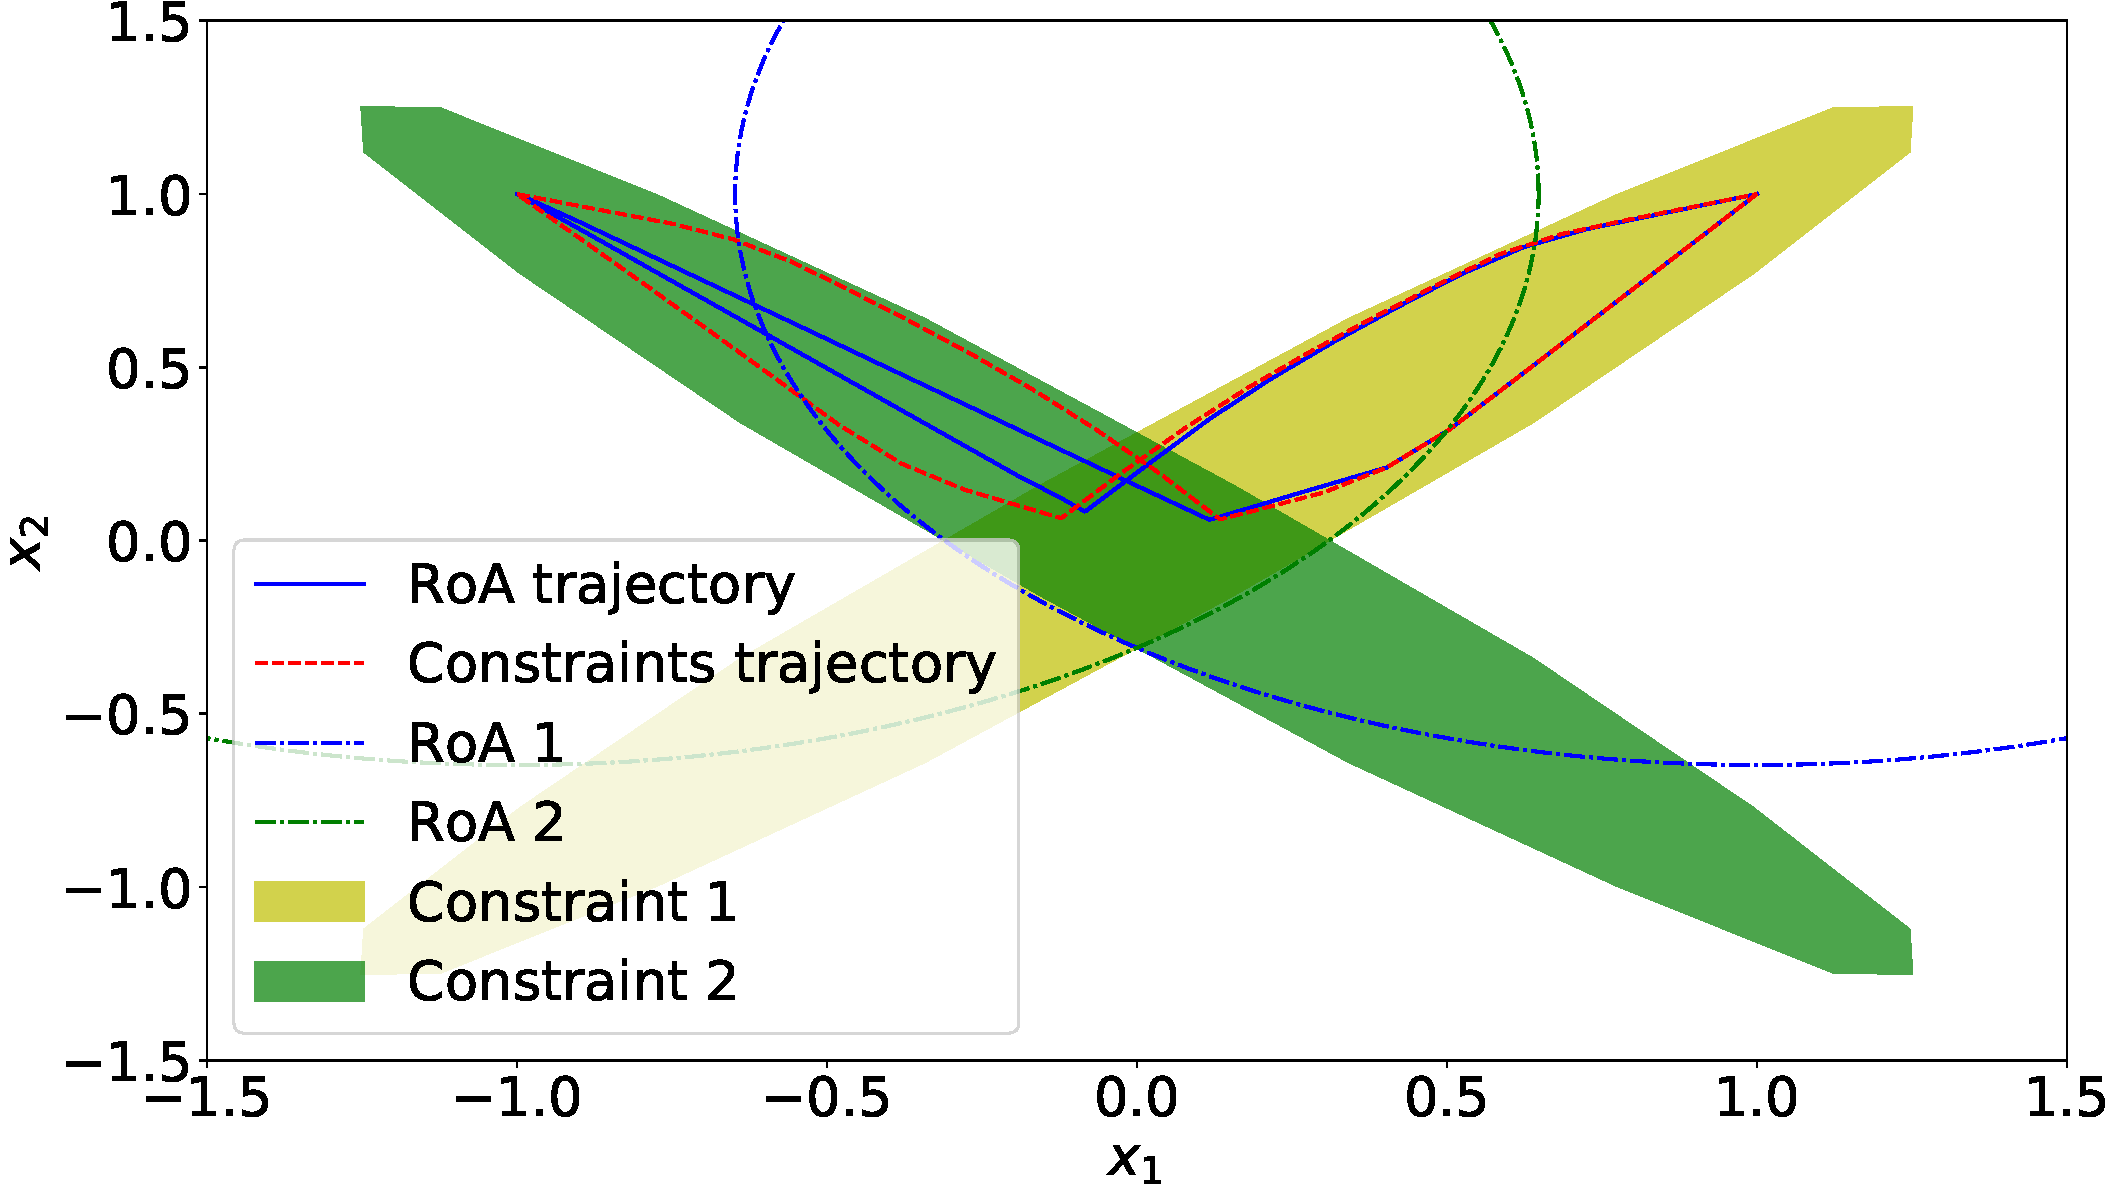
\includegraphics[height=0.75\textheight]{unstable_states}
    \caption{States trajectory for Example 2}%
    \label{fig:unstable-states}
  \end{figure}
  \vspace*{\fill}
\end{slide}

\begin{slide}{Goal of Command Governor}
  \vspace*{\fill}
  \begin{figure}[ht!]
    \centering
    \captionsetup{justification=centering}
    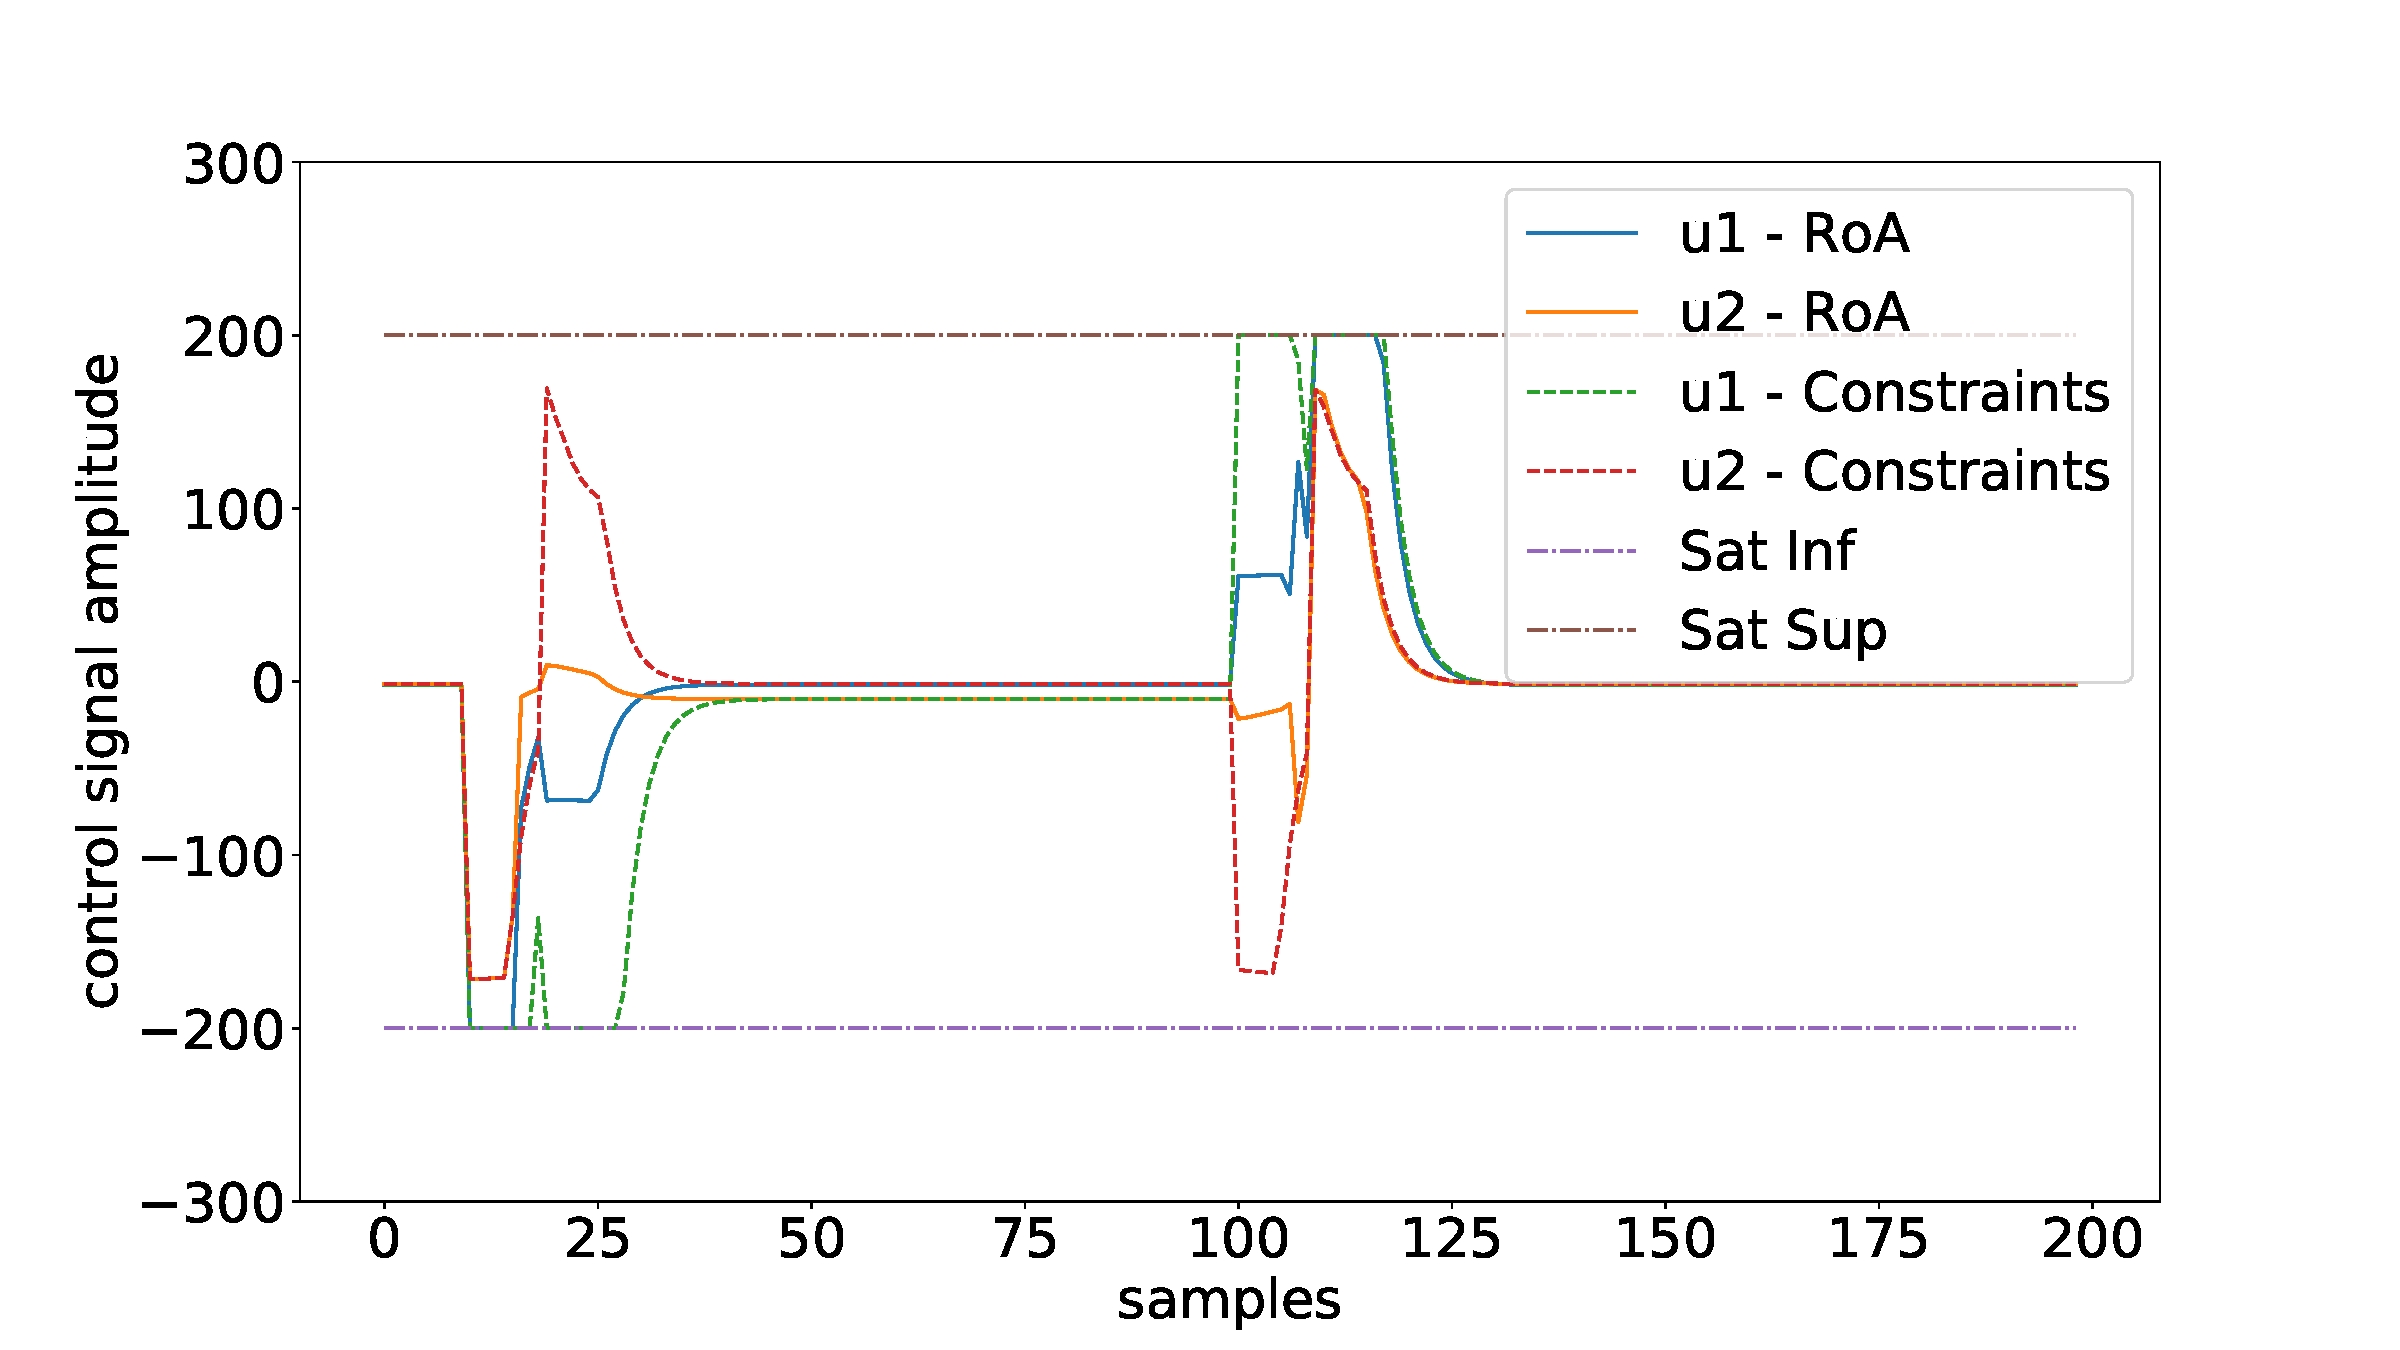
\includegraphics[height=0.75\textheight]{unstable_control_signal}
    \caption{Control signals for Example 2}%
    \label{fig:unstable-control-signals}
  \end{figure}
  \vspace*{\fill}
\end{slide}

\subsection{Cessna 182}%
\label{subsec:cessna}

\begin{slide}{Goal of Command Governor}
  \vspace*{\fill}
  \begin{figure}[ht!]
    \centering \captionsetup{justification=centering}
    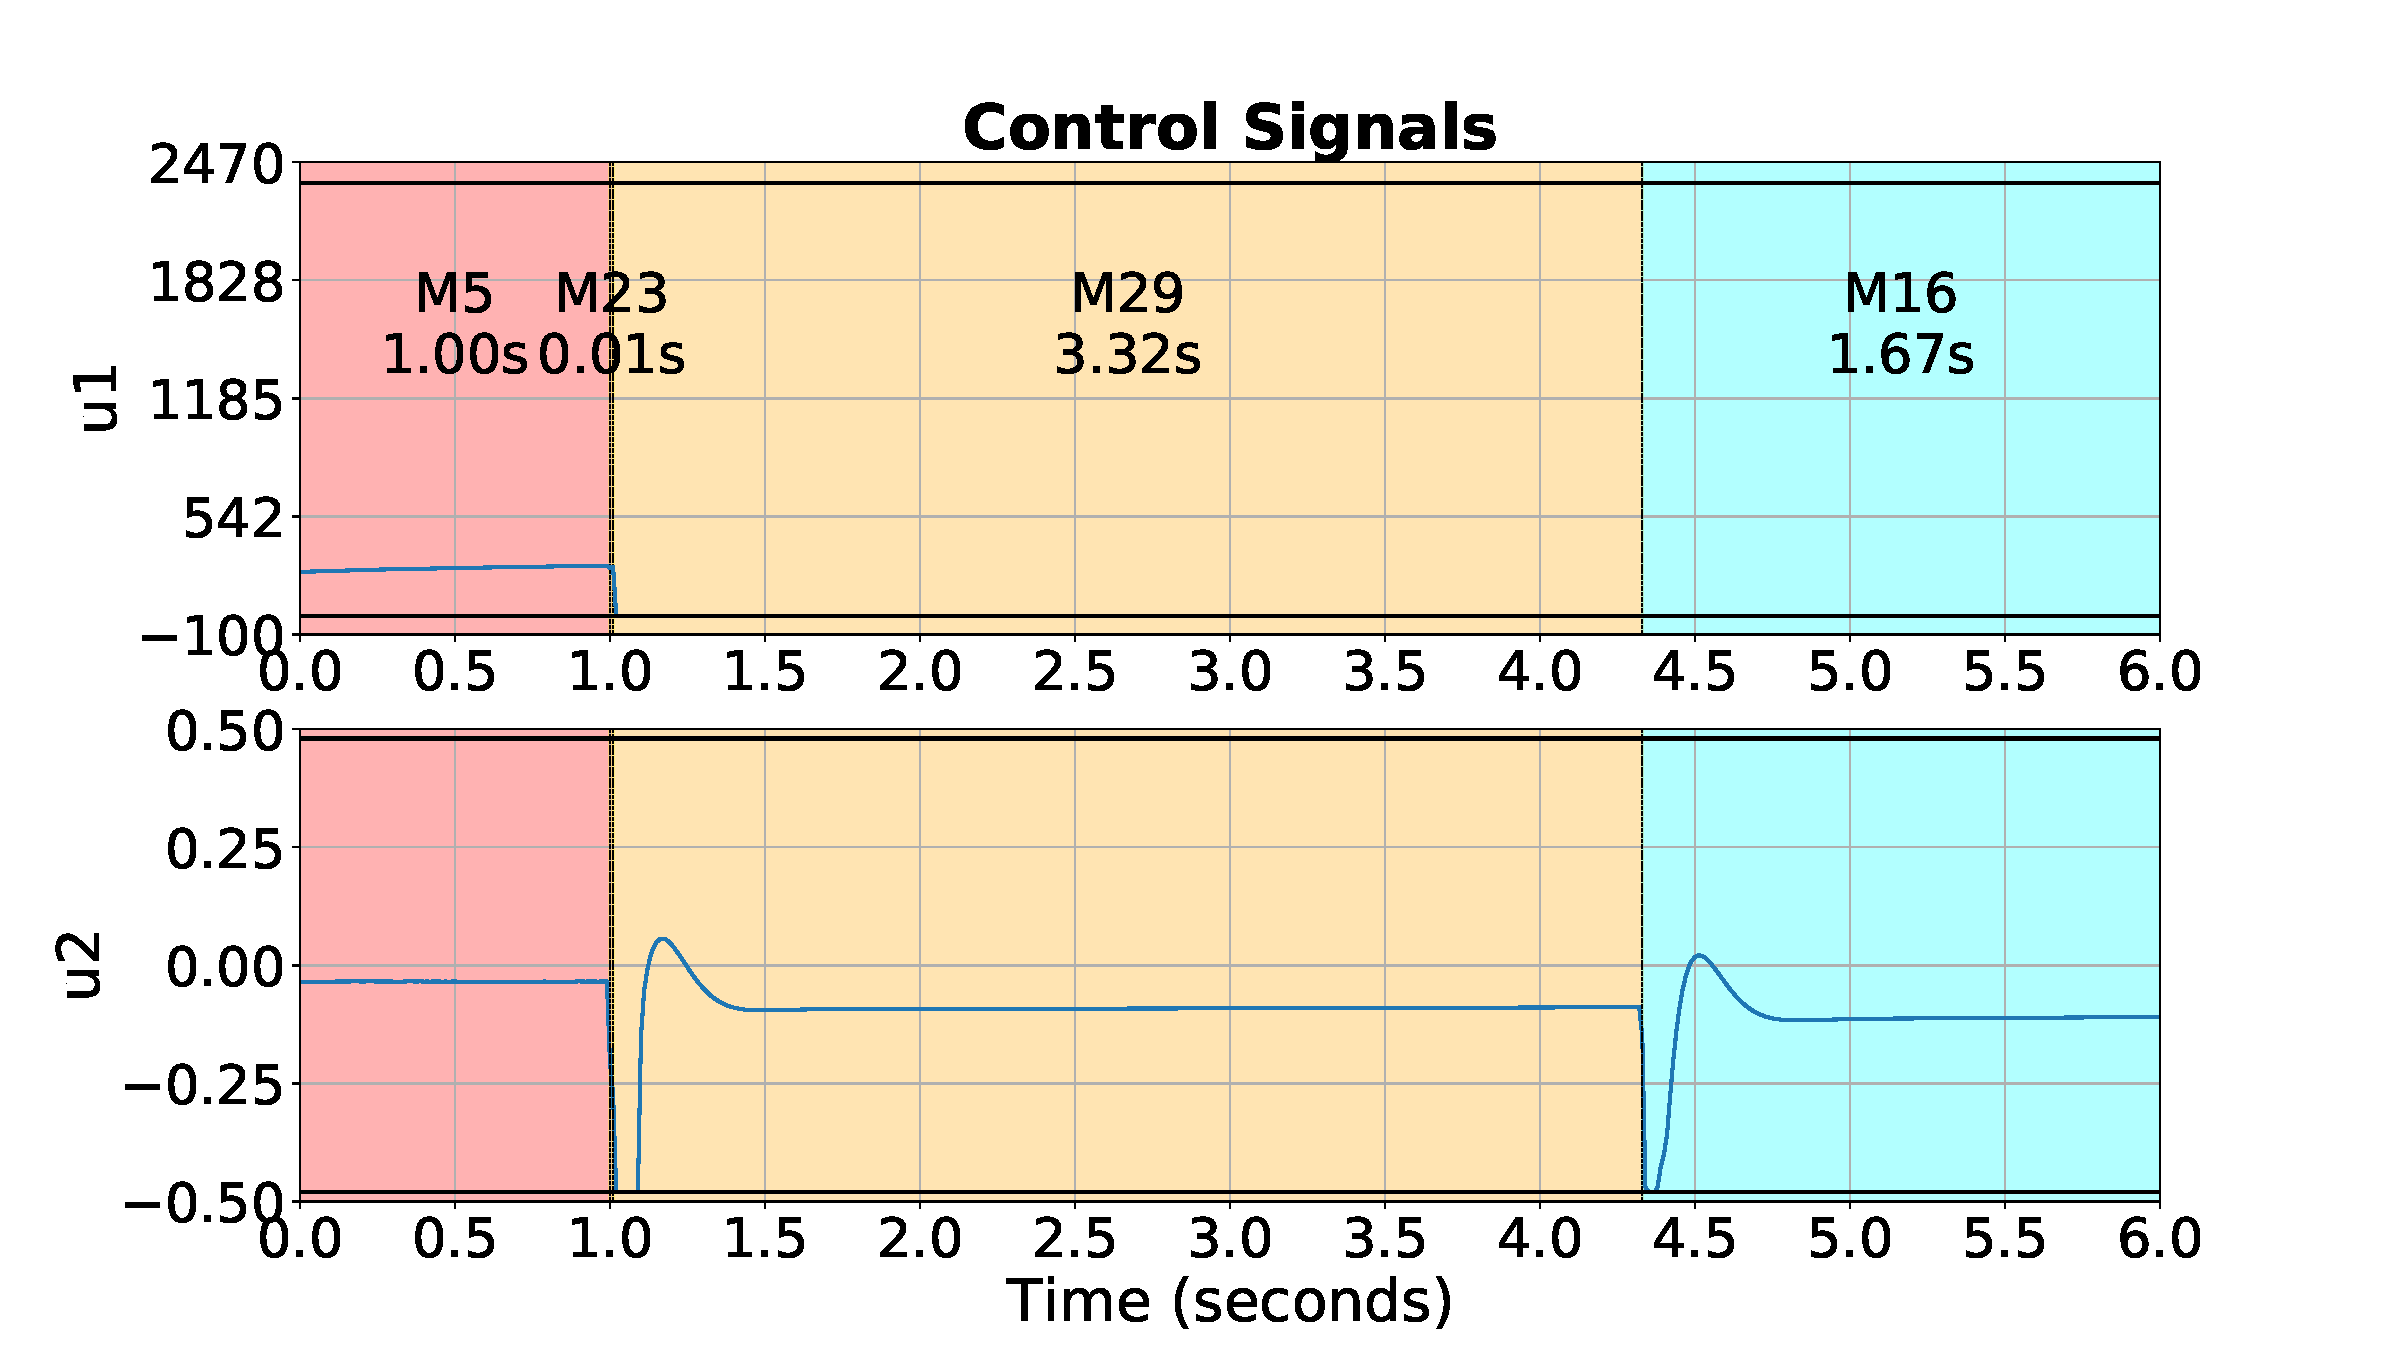
\includegraphics[height=0.75\textheight]{cessna-u}
    \caption{Cessna simulation control signal}%
    \label{fig:cessna-u}
  \end{figure}
  \vspace*{\fill}
\end{slide}

\begin{slide}{Goal of Command Governor}
  \vspace*{\fill}
  \begin{figure}[ht!]
    \centering \captionsetup{justification=centering}
    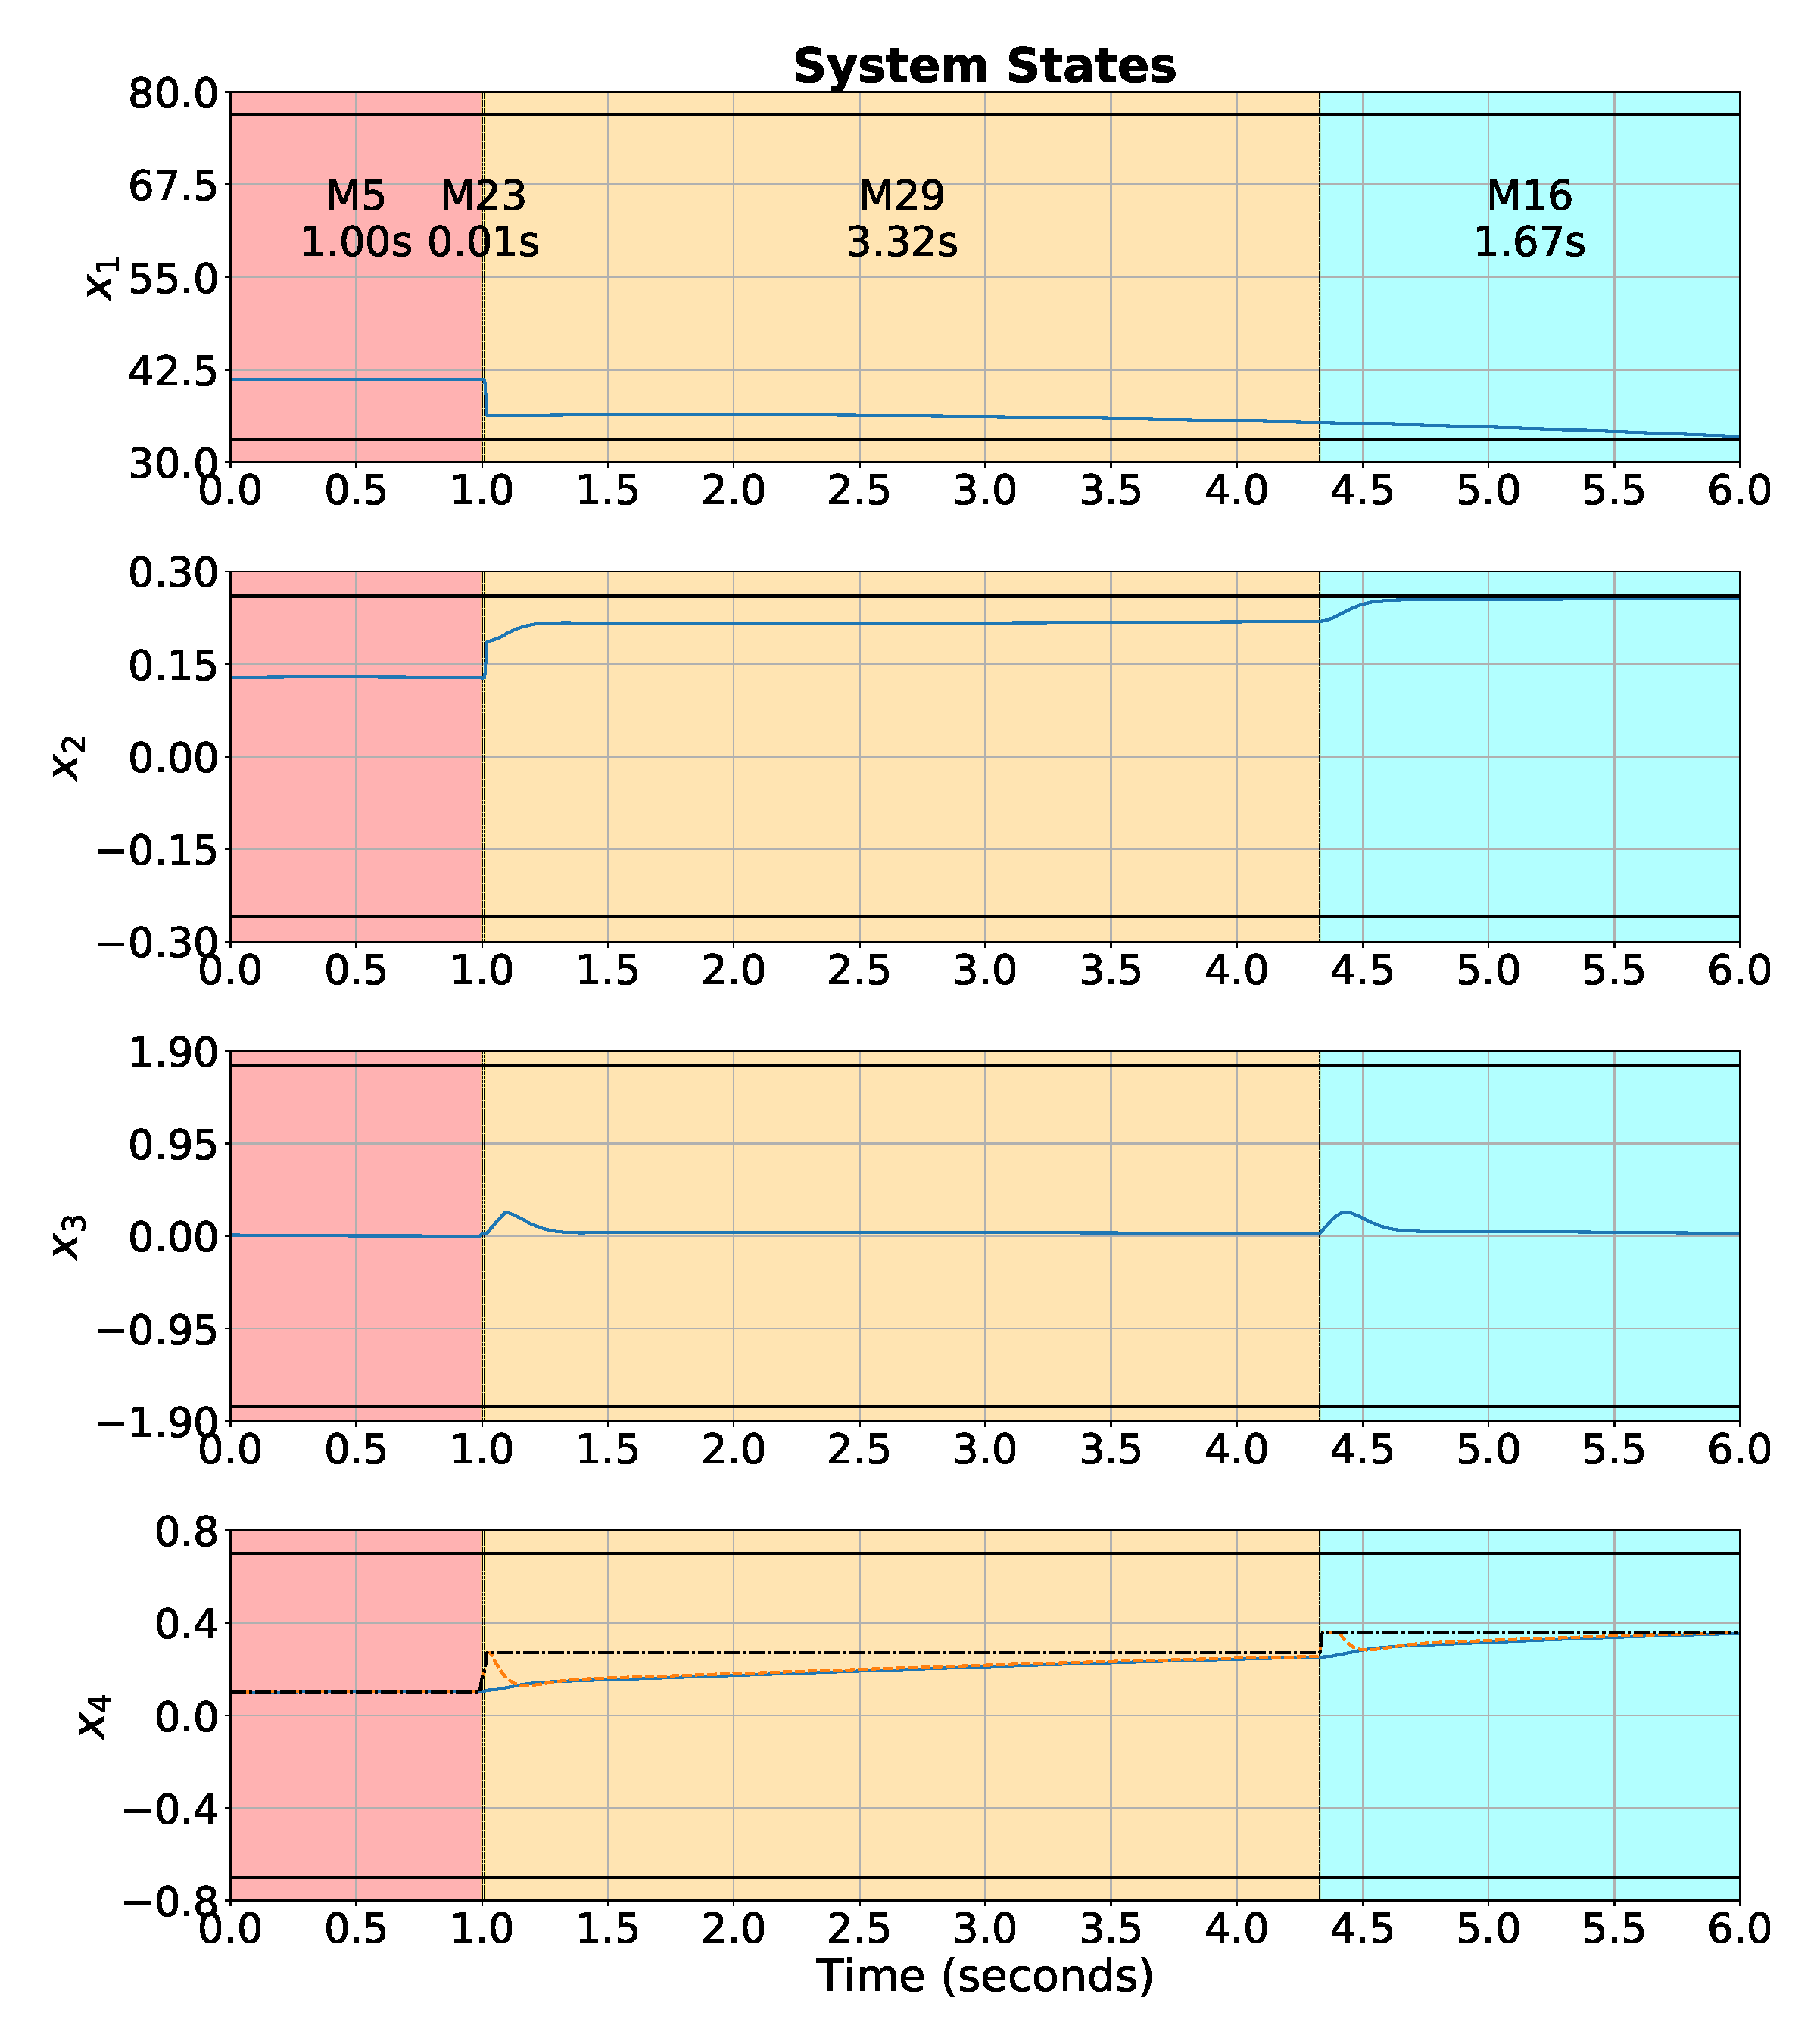
\includegraphics[height=0.75\textheight]{cessna-x}
    \caption{Cessna simulation states}%
    \label{fig:cessna-x}
  \end{figure}
  \vspace*{\fill}
\end{slide}

\subsection{Coupled Tanks}%
\label{subsec:tanks}

\begin{slide}{Goal of Command Governor}
  \vspace*{\fill}
  \begin{figure}[ht!]
    \centering \captionsetup{justification=centering}
    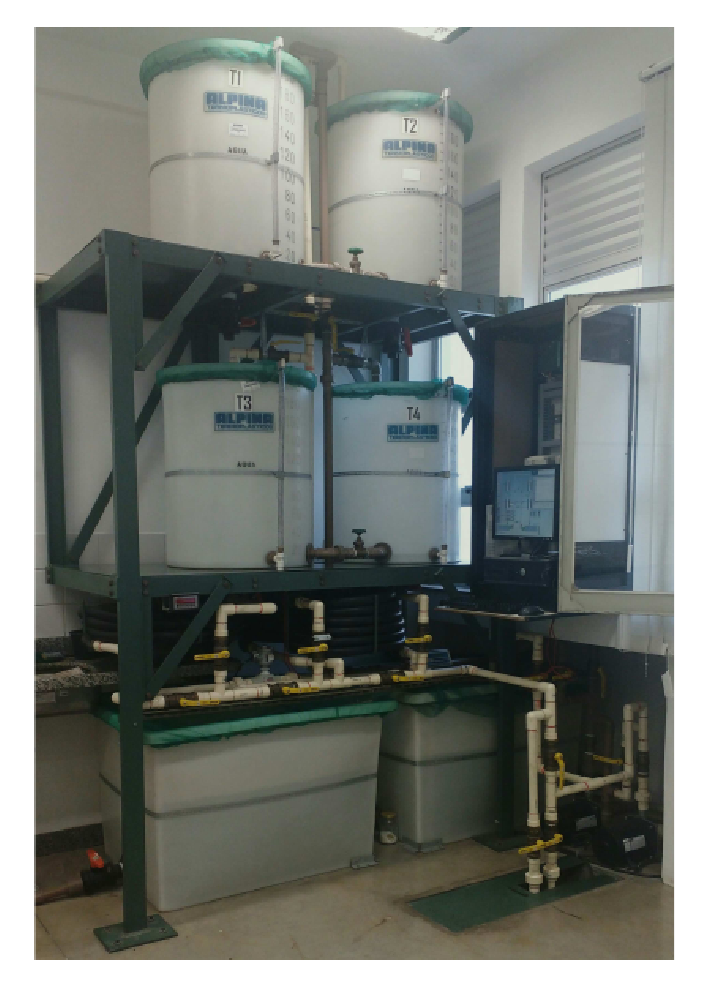
\includegraphics[height=.75\textheight]{tanks-real}
    \caption{Tank system}%
    \label{fig:tanks-real}
  \end{figure}
  \vspace*{\fill}
\end{slide}

\begin{slide}{Goal of Command Governor}
  \vspace*{\fill}
  \begin{figure}[ht!]
    \centering \captionsetup{justification=centering}
    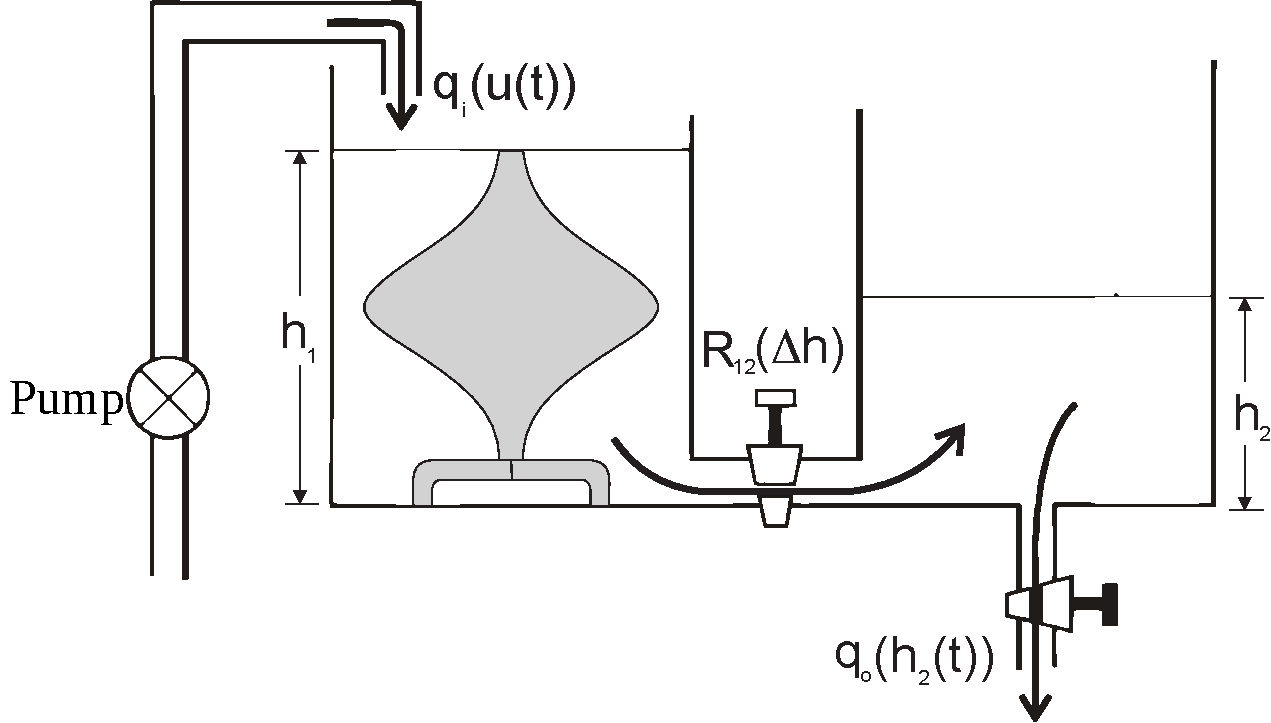
\includegraphics[height=.75\textheight]{tanks}
    \caption{Tank system diagram}%
    \label{fig:tanks}
  \end{figure}
  \vspace*{\fill}
\end{slide}

\begin{slide}{Goal of Command Governor}
  \vspace*{\fill}
  \begin{equation}
    \label{eq:t1-area}
    A_{1}(h_{1}(t)) = \frac{3r}{5} \left(
    2.7r - \frac{\cos(2.5\pi{}((h_{1}(t)-8)\times{}10^{-2}-\mu))}{\sigma{}\sqrt{2\pi}}
    e^{-\frac{((h_{1}(t)-8)\times{}10^{-2}-\mu^{2})^{2}}{2\sigma^{2}}}
    \right)
  \end{equation}
  \vspace*{\fill}
\end{slide}

\begin{slide}{Goal of Command Governor}
  \vspace*{\fill}
  \begin{equation}
    \label{eq:formula-height-variation}
    \begin{aligned}
      \dot{h}_1(t) & = \frac{R_{12}(h_{1}(t),h_{2}(t))\times{}K_{b}\times{}u(t)-h_{1}(t)+h_{2}(t)}
      {A_{1}(h_{1}(t))\times{}R_{12}(h_{1}(t),h_{2}(t))},                                                                \\
      \dot{h}_2(t) & = \frac{h_{1}(t)-h_{2}(t)}{R_{12}(h_{1}(t),h_{2}(t))\times{}A_{2}} - \frac{q_{o}(h_{2}(t))}{A_{2}}.
    \end{aligned}
  \end{equation}
  \vspace*{\fill}
\end{slide}

\begin{slide}{Goal of Command Governor}
  \vspace*{\fill}
  \begin{equation}
    \begin{aligned}
      \label{eq:op-points}
      \left[\begin{array}{c|c}
          x_{eq}^{\top} & u_{eq} \\
          \hline
          A             & B
        \end{array}\right]_{1} & = \left[\begin{array}{cc|c}
          19.5  & 5    & 15     \\
          \hline
          0.91  & 0.14 & 0.028  \\
          0.085 & 0.9  & 0.0013
        \end{array}\right], \\
      \left[\begin{array}{c|c}
          x_{eq}^{\top} & u_{eq} \\
          \hline
          A             & B
        \end{array}\right]_{2} & = \left[\begin{array}{cc|c}
          27.5  & 11.6 & 20     \\
          \hline
          0.94  & 0.19 & 0.04   \\
          0.084 & 0.9  & 0.0018
        \end{array}\right], \\
      \left[\begin{array}{c|c}
          x_{eq}^{\top} & u_{eq} \\
          \hline
          A             & B
        \end{array}\right]_{3} & = \left[\begin{array}{cc|c}
          37.3  & 17.8 & 25     \\
          \hline
          1.1   & 0.47 & 0.1    \\
          0.086 & 0.92 & 0.0042
        \end{array}\right], \\
      \left[\begin{array}{c|c}
          x_{eq}^{\top} & u_{eq} \\
          \hline
          A             & B
        \end{array}\right]_{4} & = \left[\begin{array}{cc|c}
          47.4  & 24.9 & 30     \\
          \hline
          0.49  & 0.96 & 0.22   \\
          0.053 & 0.95 & 0.0096
        \end{array}\right].
    \end{aligned}
  \end{equation}
  \vspace*{\fill}
\end{slide}

\begin{slide}{Goal of Command Governor}
  \vspace*{\fill}
  \begin{equation}
    \begin{aligned}
      K_{1} & = \begin{bmatrix} -12.884 & -97.540 & -13.975 \end{bmatrix}, \\
      K_{2} & = \begin{bmatrix} -10.054 & -73.777 & -10.523 \end{bmatrix}, \\
      K_{3} & = \begin{bmatrix} -5.840  & -31.622 & -4.148 \end{bmatrix}, \\
      K_{4} & = \begin{bmatrix} -1.832  & -21.527 & -4.177 \end{bmatrix}.
    \end{aligned}
  \end{equation}
  \vspace*{\fill}
\end{slide}

\begin{slide}{Goal of Command Governor}
  \vspace*{\fill}
  \begin{figure}[ht!]
    \centering \captionsetup{justification=centering}
    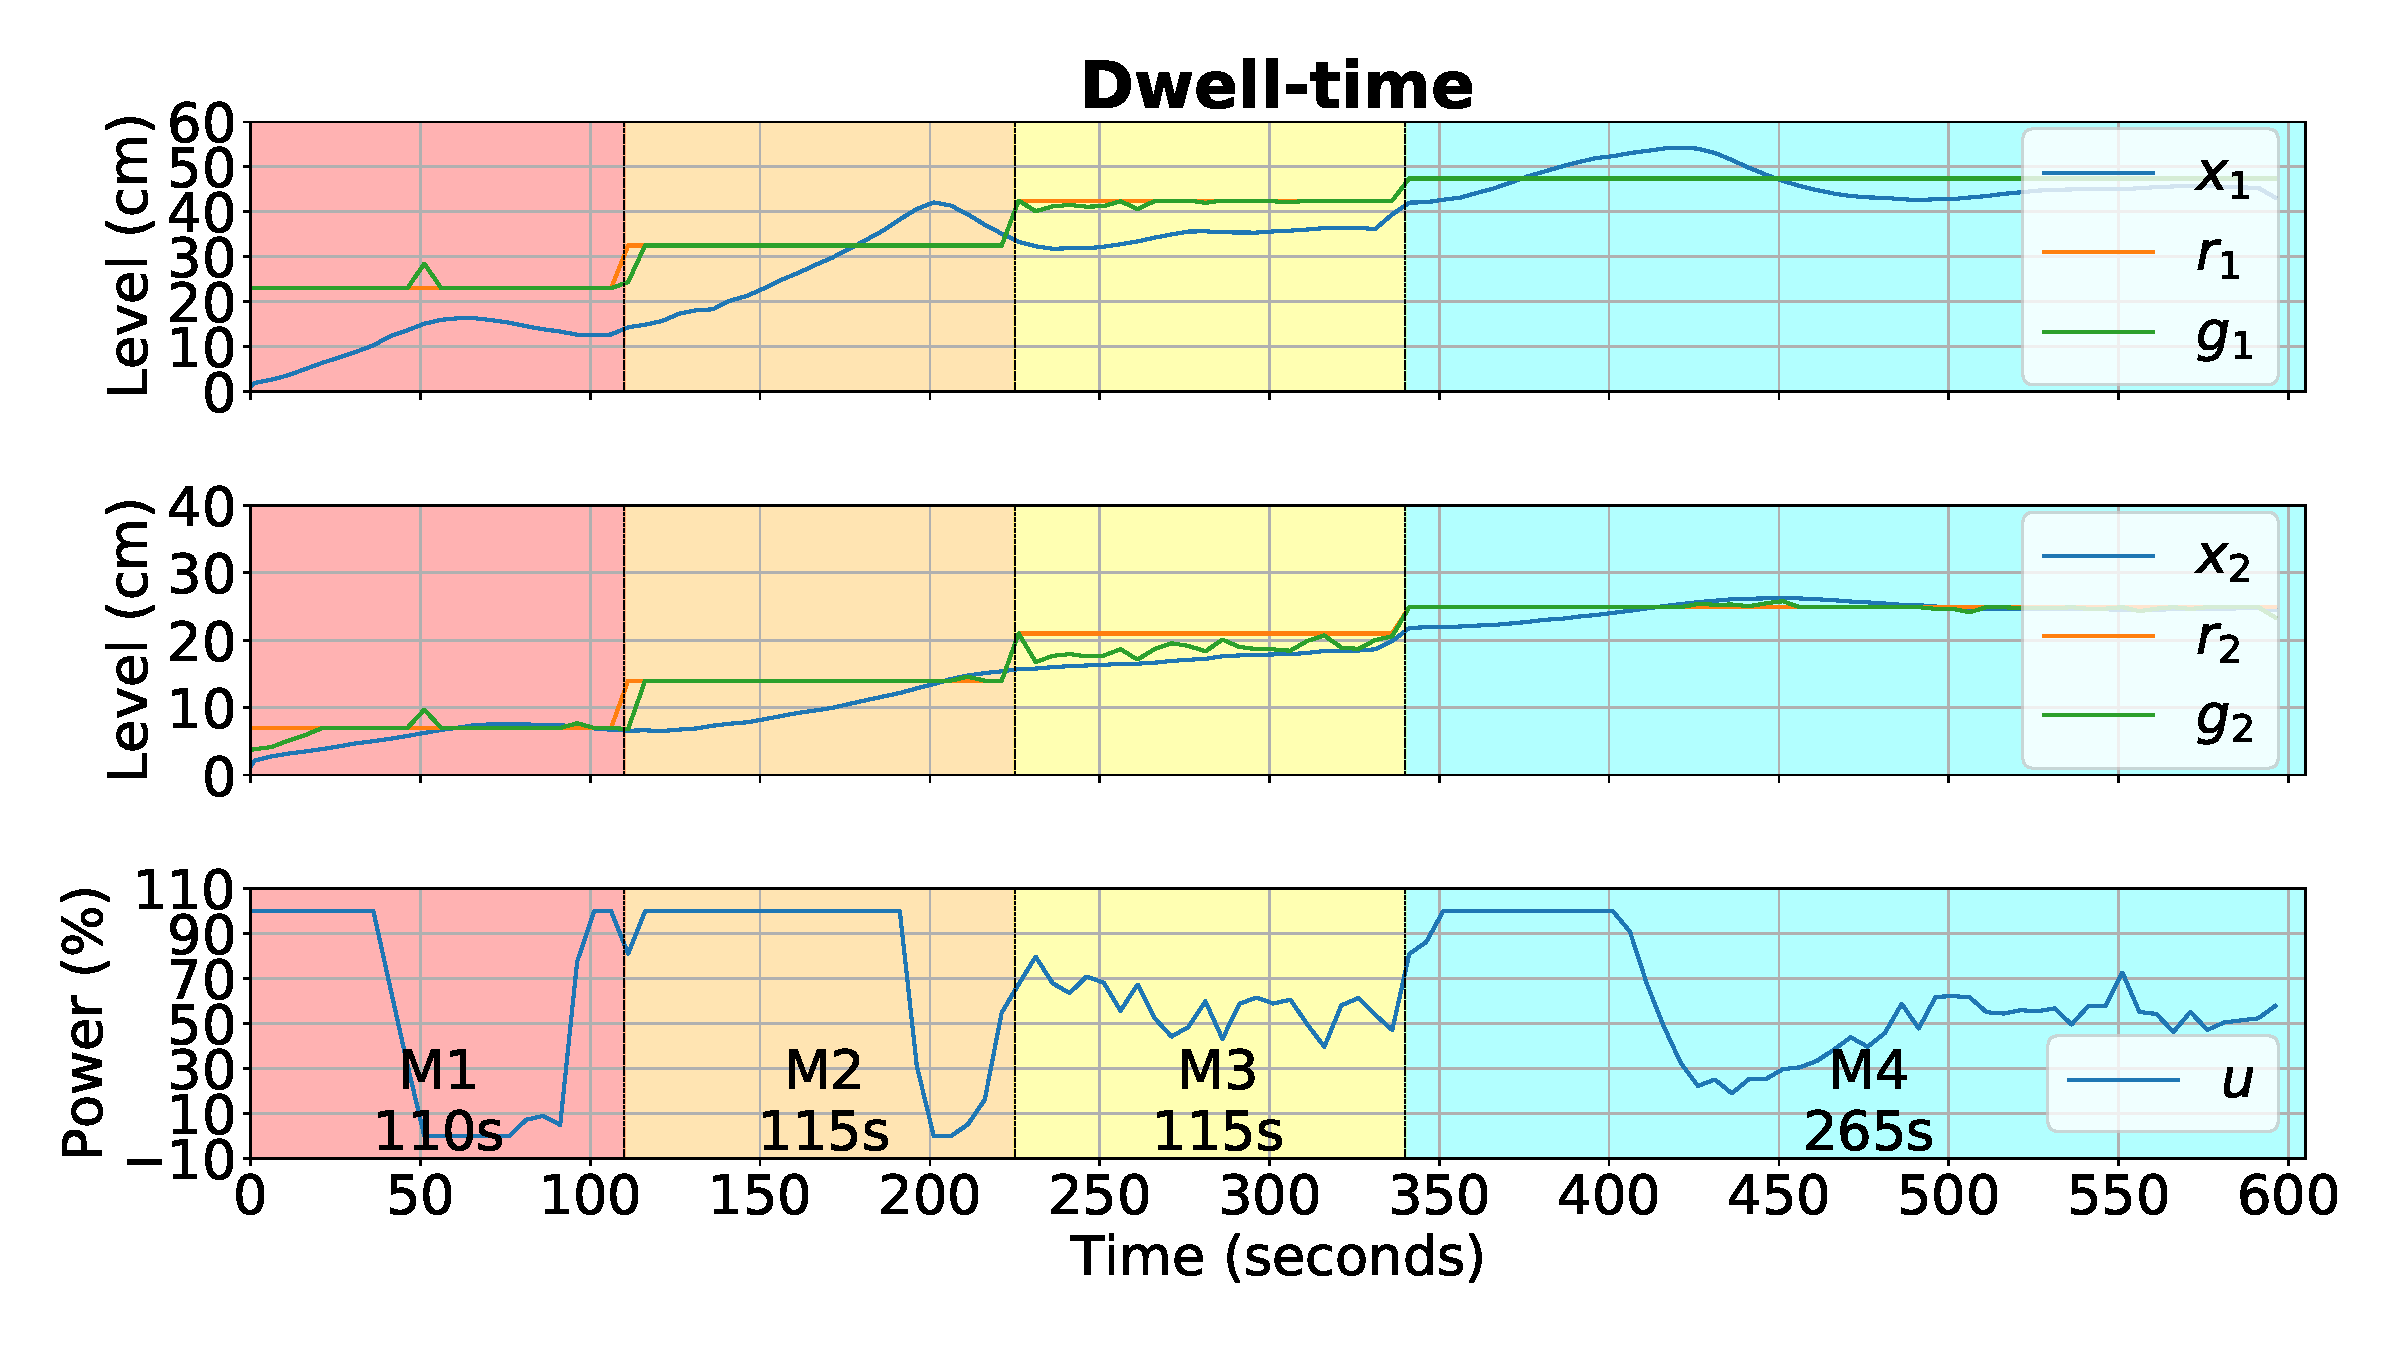
\includegraphics[width=0.7\linewidth]{tanks-dwell}
    \caption{Dwell-time approach}%
    \label{fig:tanks-dwell}
  \end{figure}
  \vspace*{\fill}
\end{slide}

\begin{slide}{Goal of Command Governor}
  \vspace*{\fill}
  \begin{figure}[ht!]
    \centering \captionsetup{justification=centering}
    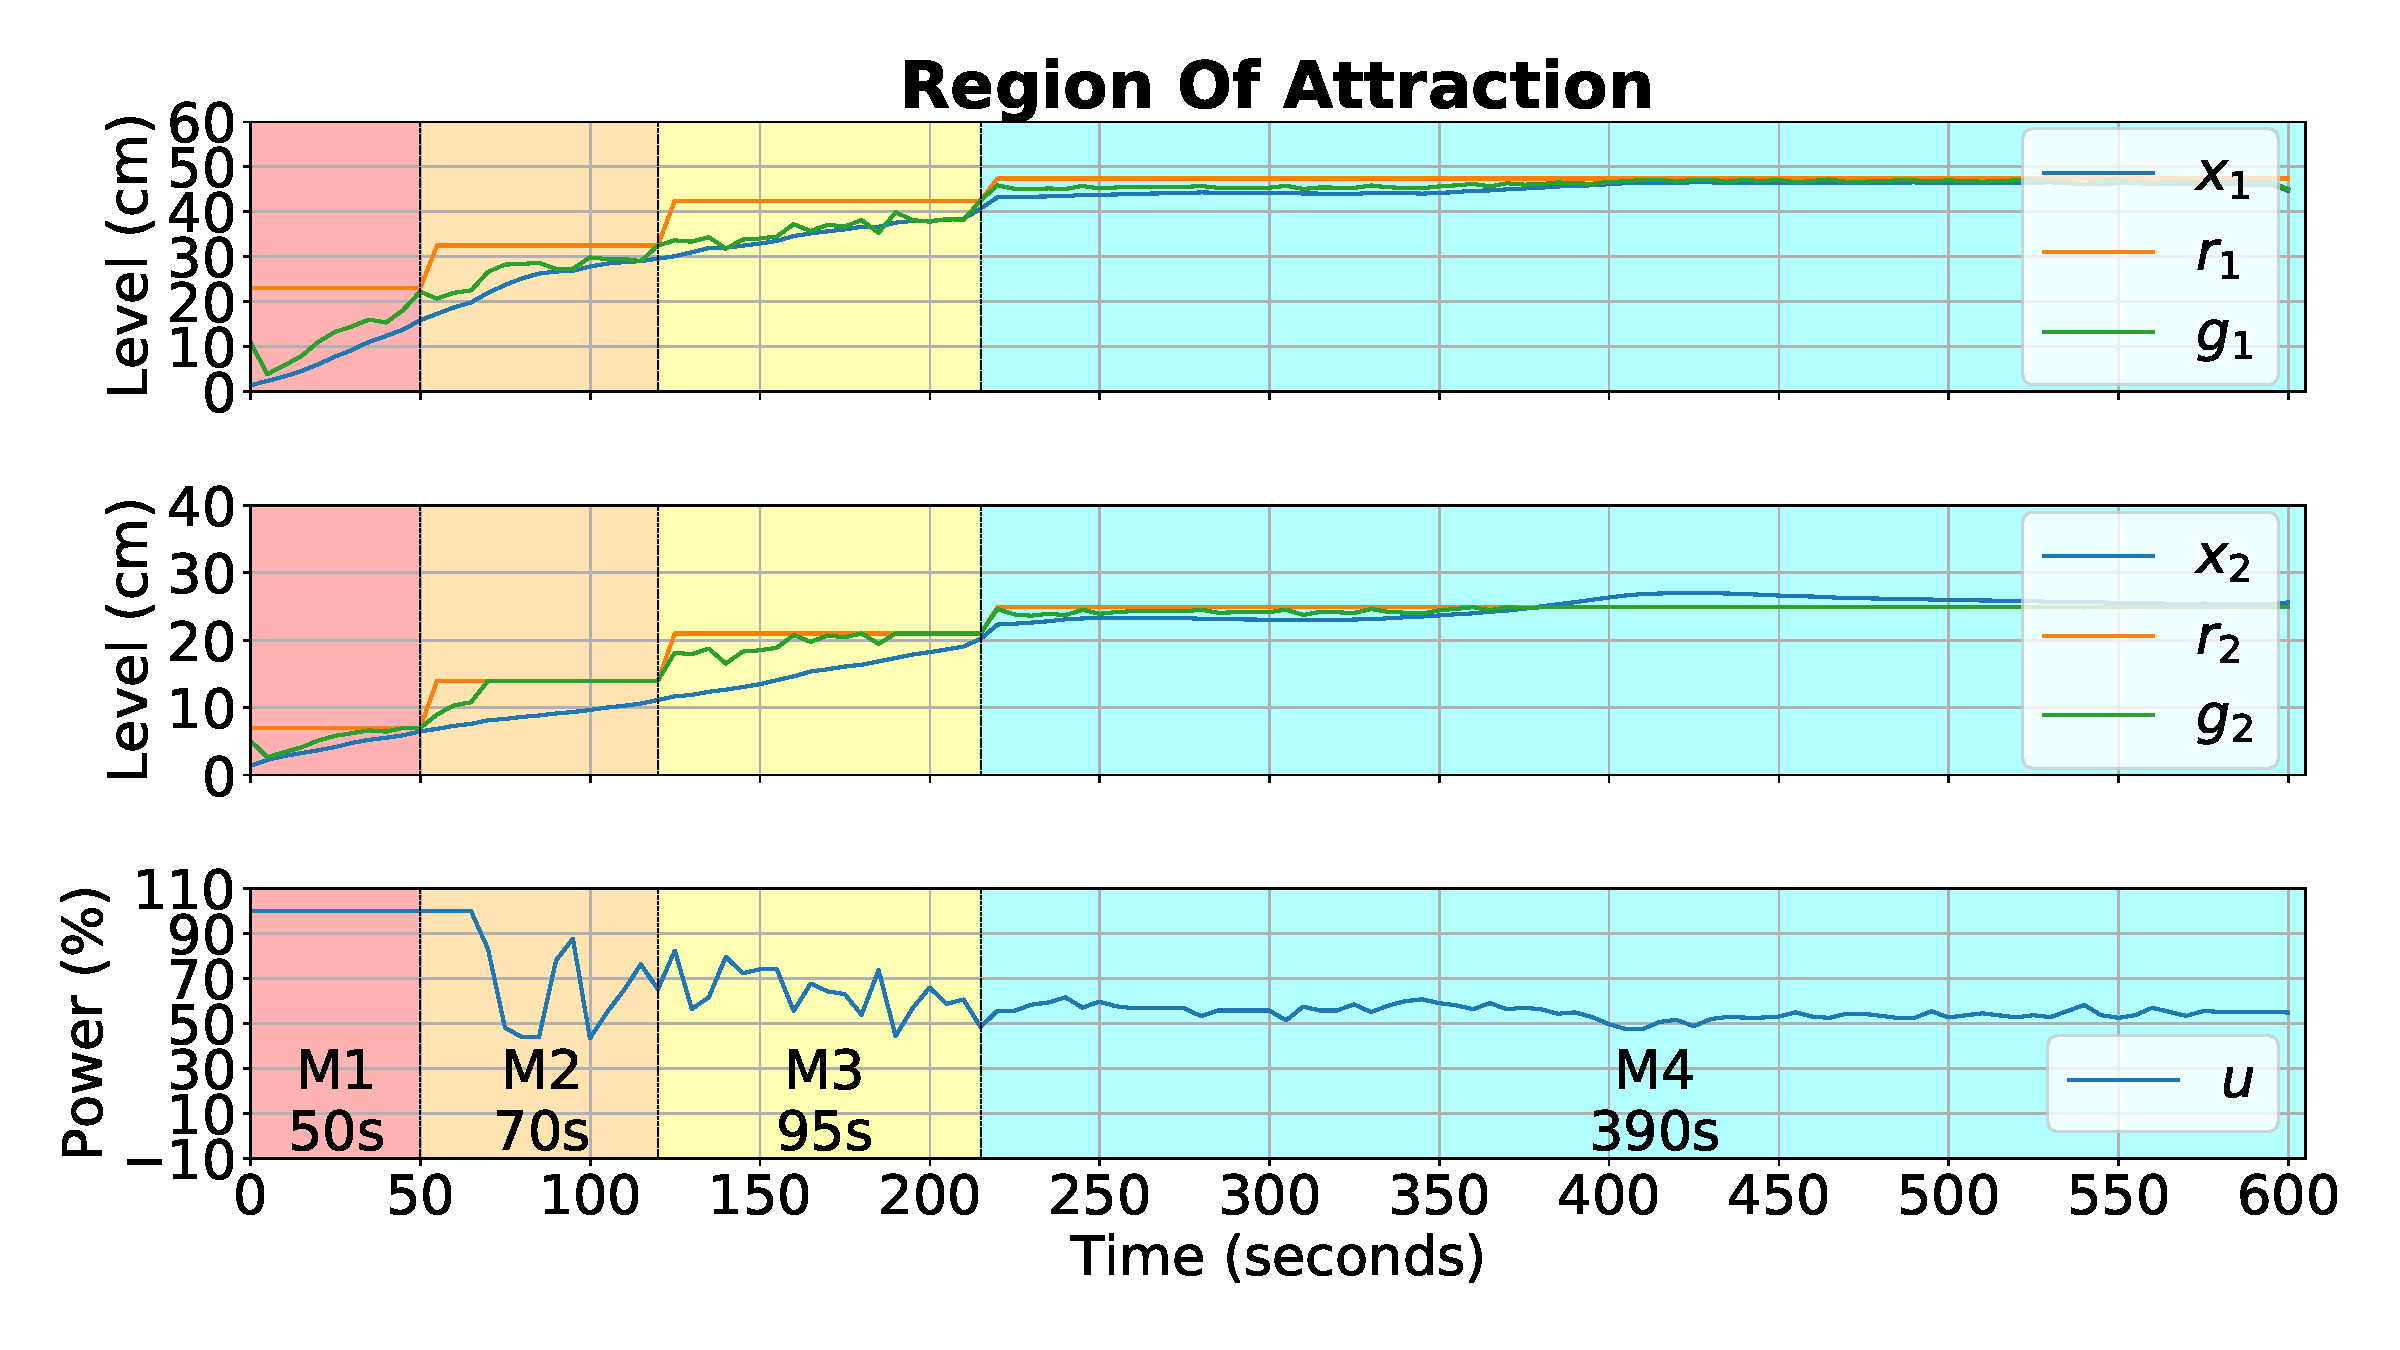
\includegraphics[width=0.7\linewidth]{tanks-roa}
    \caption{Proposed RoA-based approach}%
    \label{fig:tanks-roa}
  \end{figure}
  \vspace*{\fill}
\end{slide}
